\chapter{Introduction}
\begin{chapquote}
{Edward Witten}
``Particle physics is a modern name for the centuries old effort to understand the basic laws of physics.''
\end{chapquote}
%
% Mandatory citations: 
% aQGC thesis by Carsten Bittrich ~\cite{Bittrich2012}
%

Everybody is excited to know about the behaviour of nature around us, e.g. we are standing on earth but where the earth is standing, how it comes into existence, why there are lots of stars, and so on.
These are the general questions asked by every human being. Answers and explanations to all these question will lead us to the fundamental physics.
If we would like to understand it deeper and deeper, it will lead us to the particle physics.
As the name infers it deals with the particles (the fundamental particles) of matter and the interactions among them.

In the last century this theory was developed to describe the fundamental particles and their interactions and is known as the Standard Model (SM) of particle physics.
Up to now this theory is well tested and with the discovery of the Higgs boson the spectrum of particles predicted by it is complete.
Now the next important task is to study rigorously the precision measurement and test the deviation in the SM prediction, specially in the electroweak sector~\cite{Baak2013}.

In this chapter, first a brief introduction to SM is given then a unique way to explore the electroweak sector using the anomalous quartic gauge coupling is discussed probed by the vector boson scattering. Also, the doubly charged Higgs model, George-Machak model, is discussed. It gives multiple Higgs candidate using Higgs triplets by preserving the custodial symmetry. And in return it gives neutrino a Majorana mass.


\section{Brief Introduction of SM} % (fold)
\label{sec:brief_introduction_of_sm}
SM is the theory of elementary particles and their interactions. It is well tested and in good agreement with experimental results.

Till now we know four fundamental interactions. Out of four, the gravitational interaction is not included in SM. The other three forces the strong force interaction is described by Quantum Chromodynamics (QCD), the electromagnetic interaction is described by Quantum Electrodynamics (QED) and the weak interaction are included in the SM. In 1979 Sheldon Glashow, Abdus Salam, and Steven Weinberg awarded Nobel prize for their effort to unify the theory of weak interaction and the quantum electrodynamics. This unified theory of weak interaction and quantum electrodynamics is known as electroweak theory.

According to SM all the fundamental particles can be classified into two categories. They are fermions and bosons.

Fermions are the particles that obey the Fermi-Dirac statistics with half-integer spin. In SM fermions are further classified into leptons and quarks, which are listed in Table~\ref{table:smfermions} . Till now we know the three generations of leptons as well as quarks. The different generations are differ only in the particle mass.
\begin{table}
% \vspace{-5.2em}
\centering
\begin{tabular}[!htbp]{l l l l l l}
\hline
{\textbf{Generation}} & {\textbf{Fermion}} & {\textbf{Electric}} & \multicolumn{2}{c}{\textbf{Weak isospin $|I_3|$}} & \textbf{Mass in MeV} \\
    &           &    \textbf{Charge}  & \textbf{left-} & \textbf{right-} &     \\
    &           &                     & \textbf{handed} & \textbf{handed} &    \\
\hline
\multirow{4}{*}{$1^{st}$} & electron ($e^-$)           &   -1 & 1/2 &  0    &   0.511 \\
         & electron-neutrino ($\nu_e$)&   0  & 1/2 &  none &   $<2~.~10^{-6}$   \\
         & up quark ($u$)             &  2/3 & 1/2 &  0    &   2.3  \\
         & down quark ($d$)           & -1/3 & 1/2 &  0    &   4.8  \\
\hline
\multirow{4}{*}{$2^{nd}$} & muon ($\mu^-$)             &  -1  & 1/2 &  0    &   105.7 \\
         & muon-neutrino ($\nu_{\mu}$)& 0    & 1/2 &  none &   $<2~.~10^{-6}$   \\
         & charm quark ($c$)                & 2/3  & 1/2 &  0    &   1275     \\
         & strange quark ($s$)              & -1/3 & 1/2 &  0    &   95       \\
\hline
\multirow{4}{*}{$3^{rd}$} & tau ($\tau^-$)             & -1   & 1/2 &  0    &    1177    \\
         & tau-neutrino ($\tau_{\mu}$)& 0    & 1/2 &  none &   $<2~.~10^{-6}$   \\
         & top quark ($t$)                  & 2/3  & 1/2 &  0    &   $1.735\times 10^5$\\
         & bottom quark ($b$)               & -1/3 & 1/2 &  0    &   $4.18 \times 10^3$\\
\hline
\end{tabular}
\caption{Fermions list in SM~\cite{Bittrich2012}.}
\label{table:smfermions}
\end{table}

Bosons are the particles that obey the Bose-Einstein statistics with integer spin. In SM the bosons are the mediator of interactions between the particles, described by local gauge theory. Thus, these bosons are called gauge bosons. All the bosons in SM are listed in Table~\ref{table:smbosons}. The photon and gluons are massless carrying electromagnetic and strong force respectively. The $W^{\pm}$ and $Z$ bosons carry the weak force. These bosons are the spin 1 bosons and known as the vector-bosons. Whereas, the Higgs boson, H, is a scalar boson with spin 0.

\begin{table}
% \vspace{-5.2em}
\centering
\begin{tabular}[!htbp]{l l l l l l}
\hline
    & \textbf{Bosons} & \textbf{Electric Charge} & \textbf{Spin} & \textbf{Interaction} & \textbf{Mass in GeV} \\
\hline
$\gamma$  & photon   & 0      & 1 & electromagnetic   &   $<1~.~10^{-27}$ \\
$W^{\pm}$ & W bosons & $\pm$1 & 1 & weak              &  80.385     \\
$Z^0$     & Z boson  & 0      & 1 & weak              &  91.188     \\
$g$       & gluons   & 0      & 1 & strong            &  0          \\
\hline
$H$       & Higgs    & 0      & 0 &                    & 125        \\
\hline
\end{tabular}
\caption{Bosons list in SM~\cite{Bittrich2012}.}
\label{table:smbosons}
\end{table}

\subsection{Standard Model as Gauge theory}
% The concept of gauge invariance is fundamental in the construction of the Standard Model of strong, weak and electromagnetic interactions of elementary particles. The gauge principle prescribes that, given the gauge symmetry group and the transformations of the fields, the quantum field theory is uniquely defined [@book:CoughlanDodd].
QED is a local gauge theory because the Lagrangian function that describes it remains unchanged by the following local gauge transformation of the electron field $\psi(x)$ and the photon field $A_\mu(x)$ at all space-time point x:
\begin{eqnarray}
    \psi(x) & \rightarrow & e^{ie\Lambda(x)}\psi(x), \nonumber \\
    A_\mu(x) & \rightarrow & A_\mu(x) + \frac{\partial \Lambda(x)}{\partial x_\mu}, \nonumber
\end{eqnarray}
with arbitrary $\Lambda(x)$, where e is the electron-photon coupling (other charged spin-$\frac{1}{2}$ fields transform similarly to $\psi$). The photon field plays an intrinsic part; there could be no local gauge invariance without it. Hence if we take the postulate of this local gauge invariance for spin-$\frac{1}{2}$ particles as a starting point, the existence of gauge boson is required and in fact their coupling to fermions is specified, too. For exact gauge invariance the gauge bosons must be massless.

The phase factor $e^{i\Lambda(x)}$ belong to the symmetry group $U(1)$ of unitarity transformations in one dimension. The generalization of QED to other forces is made by looking for other possible symmetry groups and using them as the basis of more general gauge transformations. 
        
For example, we may choose to regard the electron and neutrino as a doublet $(\nu_e,e)$, i.e. as two members of the same family, since both are light spin-$\frac{1}{2}$ particles. We can then describe this doublet by a two component field $\psi = (\psi_\nu,\psi_e)$ and introduce gauge transformations where $\Lambda$ is a $2\times 2$ hermitian matrix operating on $\psi$.  We can put the other leptons and the quarks, too, in doublets $(\nu_\mu,\mu),(\nu_\tau,\tau),(u,d),etc.$ and subject them to similar gauge transformations. These transformations are much more than phase factors, since the off-diagonal elements of $\Lambda$ can change one member of a doublet into the other; they belong to the symmetry group SU(2) of unitary unimodular transformations in two dimensions. Local gauge invariance in this case requires the introduction of three massless spin-1 gauge bosons $W^+,W^-$ and $W^0$. If this is combined with a simultaneous U(1) symmetry (bringing one more gauge boson $B^0$), we get the $SU(2)_L\times U(1)$ Glashow-Salam-Weinberg theory of electroweak interactions [article:weinberg]. The gauge bosons can not all be massless, experiment excludes this, so the symmetry can not be exact. The symmetry is broken spontaneously, in a way that retains renormalizability; the result is one massless gauge boson $\gamma$ (made from a linear combination $W^0sin\theta_w +B^0cos\theta_w$) plus three massive gauge bosons $W^+, W^-$ and $Z^0$ (the orthogonal combination $W^0cos\theta_w - B^0sin\theta_w$). The angle $\theta_w$ is a parameter of this unified electroweak theory.

The subscript L on $SU(2)_L$ above indicates that the $SU(2)$ gauge transformations operate only on left-handed particles. This is because processes like beta-decay are observed to involve quarks and leptons with left-handed spins relative to their motions. The remaining right-handed spins relative to their motions singlets that do not change under $SU(2)_L$ gauge transformations; for anti-quark and anti-leptons, interchange L and R. The first-generation spin-$\frac{1}{2}$ particles can be classified in doublet and singlet representations of $SU(2)_L$ as follows:
\begin{eqnarray}
    (u_L,d_L),(\nu_{eL},e_L),\bar{u}_L,\bar{d}_L,\bar{e}_L, \nonumber \\
    (\bar{d}_R,\bar{u}_R),(\bar{e}_R,\bar{\nu}_{eR}),u_R,d_R,e_R.   \nonumber
\end{eqnarray}
There is no right-handed neutrino state here; there is no need for such states to exist if the neutrino is massless. Thus we have 15 left-handed (and 15 right-handed) fermion states in each generation counting three colors for each quark flavor, in this gauge theory of electroweak interactions.

% <!-- %In chiral theories, where gauge bosons have different couplings to left and right handed fermion states a new problem arises- typically for the interaction of three gauge bosons via a closed loop of fermions as shown in figure
% %add figure
% %When the L and R fermion couplings are unequal at one (or three) of the vertices, as is the case in the standard electroweak theory -->

In strong interactions since each quark has three possible colors, we can describe any particular quark flavor by a three-component field $\psi(x)=[\psi(red,x),\psi(blue,x),\psi(green,x)]$ and can consider local gauge transformations where $\Lambda(x)$ is a $3\times 3$ hermitian matrix operating on $\psi$. The transformation can change the color; they belong to the symmetry group SU(3). To achieve local gauge invariance in this case requires the introduction of eight massless gauge bosons which carry pairs of color labels and are known as gluons. This gauge theory is known as QCD. Combining with the electroweak interaction gives an $SU(3)\times SU(2) \times U(1)$ gauge invariant theory of the strong and electroweak forces, commonly called the Standard Model.

With each of these gauge groups $(SU(3),SU(2)$ and $U(1))$ there is associated a characteristic coupling strength $\alpha_3,~\alpha_2,~\alpha_1$ analogous to the fine-structure constant $\alpha$ of electrodynamics. They are generally called the running couplings because their numerical values change logarithmically with the energy scale of the interaction due to renormalization.

These renormalizable gauge theories allow the presence of spin 0 (scalar) particles, too [article:higgs]. The usual formulation of the Standard Model requires at least one of these, the Higgs scalar boson, arising from the mechanism for spontaneously breaking the $SU(2)\times U(1)$ electroweak symmetry and giving masses to the weak gauge bosons and to the leptons and quarks. This mechanism is a vital part of the SM.

\subsection{Brief Introduction to Higgs Mechanism} % (fold)
\label{sub:brief_introduction_to_higgs_mechanism}\
The one of main issue with the electroweak theory was that all the particles were assumed to be massless.
The mass term was not invariant under the local gauge transformation under $SU(2)_L \times U(1)_Y$ and therefore breaks symmetry.
This issue was solved by the Higgs mechanism.
The Higgs mechanism predicts a symmetrical Higgs field having non-invariant lowest energy state. This gives mass to the fermions and boson by interacting with the Higgs field. The Higgs field can only be observed via its excitation known as the Higgs boson, H. In this section the Higgs mechanism is briefly described.
% If the broken direction in symmetry space also corresponds to a gauge symmetry (i.e. a space-time dependent symmetry) then the associated Goldstone boson and the massless gauge boson combine to form a massive gauge boson -- \textbf{the Higgs mechanism}~\cite{Chanowitz1988}

The electroweak theory contains $SU(2)_L \times U(1)_Y$ symmetry and the Higgs part of full Lagrangian is given by
\begin{equation}
    L_H=(D_{\mu}\Phi)^{\dagger}(D^{\mu}\Phi)-V(\Phi)
\end{equation}
of the SM Lagrangian extends the experimentally well established particle content of the SM by the complex scalar SU(2) doublet $\Phi = (\phi^{+},\phi^0)^T$ of weak hypercharge $Y_{w,\Phi}=1$, so that $\phi^{+}$ carries charge +e and $\phi^0$ is neutral. In total $\Phi$ involves four degree of freedom. The self-interaction of $\Phi$ is described by the potential
\begin{equation}
    V(\Phi)=-\mu^2(\Phi^{\dagger}\Phi)+\frac{\lambda}{4}(\Phi^{\dagger}\Phi)^2,
\end{equation}
Here, the term $\lambda > 0$ ensures that the potential is bounded form below. Here we need to generate masses for the three gauge bosons $W^{\pm}$ and Z but the photon should remain massless. Therefore, we needs at least 3 degree of freedom for the scalar fields. The simplest choice is a complex SU(2) doublet of scalar field $\phi$:
\begin{equation}\label{mat2}
    \Phi=
        \begin{bmatrix}
        \phi^+  \\
        \phi^0  \\
        \end{bmatrix}
    =\frac{1}{\sqrt{2}}
        \begin{bmatrix}
        \phi_1 + i\phi_2    \\
        \phi_3 + i\phi_4    \\
        \end{bmatrix}
\end{equation}
where $\phi_i$ are 4 real scalar fields (4 degree of freedom). The Lagrangian is invariant under the local gauge transformations \footnote{The concept of gauge invariance is fundamental in the construction of the Standard Model of strong, weak and electromagnetic interactions of elementary particles. The gauge principle prescribes that, given the gauge symmetry group and the transformations of the fields, the quantum field theory is uniquely defined~\cite{Coughlan2006}.}
\begin{equation}
    \Phi (x) \rightarrow \Phi(x)`=e^{i\alpha_i(x)\tau_i /2}\Phi(x)
\end{equation}
where $\tau_i$ are Pauli matrices and $\alpha_i(x)$ are transformation parameters.
Now the product
\begin{equation}\label{eq:mat1}
    \Phi{\dagger}\Phi=
        \begin{bmatrix}
        \phi^{+*}   &   \phi^{0*} \\
        \end{bmatrix}
        \begin{bmatrix}
        \phi^+  \\
        \phi^0  \\
        \end{bmatrix}
    =\phi^{+*} \phi^+ + \phi^{0*}\phi^0
    =\frac{1}{2}(\phi^2_1+\phi^2_2+\phi^2_3+\phi^2_4)
    =\frac{1}{2}\phi_i \phi^i
\end{equation}
    
For $\mu^2<0$, corresponds to the ``\textit{Maxican Hat}'' potential shown in Fig.~\ref{fig:higgsPotential}, the potential $V(\Phi)$ has a minimum at
\begin{equation}
    \Phi^{\dagger}\Phi = -\frac{\mu^2}{2\lambda}=\frac{v^2}{2}
\end{equation}
from equation~\ref{eq:mat1}, we can know that there is an infinite number of possible solutions of this equation. To preserve electric charge conservation ($U(1)_{QED}$ symmetry), this non zero vacuum expectation value should not be reached in the charged direction. A conveninent choice of the neutral direction is $\phi_1 = \phi_2 = \phi_4 = 0$. So, the equation~\ref{mat2}:
\begin{equation}
    \Phi=\frac{1}{\sqrt{2}}
        \begin{bmatrix}
        0   \\
        \phi_3  \\
        \end{bmatrix}
\end{equation}
\begin{figure}[!htbp]
    \centering
    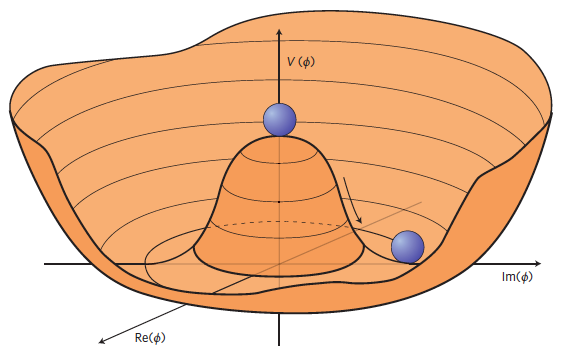
\includegraphics[width=0.45\textwidth]{figures/Intro/higgspotential.png}
    \caption{Higgs potential}
    \label{fig:higgsPotential}
\end{figure}
Therefore, the neutral component ($\phi_3$) of the doublet field $\Phi$ develops a nonzero vacuum expectation value
\begin{equation}
    {\Braket\Phi}_0 = \Braket{0|\Phi|0}=\frac{1}{\sqrt{2}}
        \begin{bmatrix}
        0   \\
        v   \\
        \end{bmatrix}
        with~
        v=-
        \begin{bmatrix}
        \frac{\mu^2}{\lambda}
        \end{bmatrix}
        ^{1/2}
\end{equation}
Now by using the unitarity gauge\footnote{It removes the unphysical degree of freedom} means of proper gauge transformation of the field we get
\begin{equation}
    \Phi (x)=\frac{1}{\sqrt{2}}
        \begin{bmatrix}
        0   \\
        v+h(x)  \\
        \end{bmatrix}
\end{equation}
With $\Phi(x)$ we can expand kinetic term $D_\mu \Phi)^{\dagger} (D_\mu \Phi)=|D_\mu \Phi|^2$ of lagrangian
\begin{eqnarray}\label{mat3}
    |D_{\mu} \Phi|^2 & = & |(\partial_{\mu}-ig_2\frac{\tau_a}{2}W^a_{\mu}-ig_1 \frac{Y_H}{2}B_{\mu})\Phi|^2 \nonumber \\
            & = & \frac{1}{2}(\partial_\mu H)^2+\frac{1}{8}g^2_2(v+H)^2|W^1_{\mu}+iW^2_\mu|^2+\frac{1}{8}|g_2W^3_\mu-g_1B_\mu|^2
\end{eqnarray}
Lets define the new fields $W^{\pm}_\mu$ and $Z_\mu$ [$A_\mu$ is the field orthogonal to $Z_\mu$]:
\begin{equation}
    W^{\pm}=\frac{1}{\sqrt{2}}(W^1_\mu \mp iW^2_\mu),~Z_\mu=\frac{g_2W^3_\mu-g_1B_\mu}{\sqrt{g^2_2+g^2_1}},~A_\mu=\frac{g_2W^3_\mu+g_1B_\mu}{\sqrt{g^2_2+g^2_1}}
\end{equation}
Now pic the term from equation~\ref{mat3} which are bilinear in the fields $W^\pm,Z,A$:
\begin{equation}
    M^2_wW^+_\mu W^{-\mu},~\frac{1}{2}M^2_z Z_\mu Z^\mu,~and~\frac{1}{2}M^2_AA_\mu A^\mu
\end{equation}
Then we noted that W and Z boson have acquired masses, while the photon is still massless
\begin{equation}
    M_w=\frac{1}{2}vg_2,~M_z=\frac{1}{2}v\sqrt{g^2_2+g^2_1},~M_A=0
\end{equation}
So, by spontaneously breaking the symmetry, three Goldstone bosons have been absorbed by the $W^{\pm}$ and Z boson to form their longitudinal components and to get their masses. Since the U(1) symmetry is still unbroken, the photon which is its generator, remains massless.

Now we established that the Higgs mechanism generates the mass for the vector boson. So, now it following the nature. But for the Higgs mechanism to be validated Higgs boson should be found experimentally. In July 2012, we found a Higgs like boson. But, is it the Higgs of SM or something else we can say now because of the uncertainty and statistical error involved in the present analysis. 

So, What are the possible ways to investigate it?

Basically there are two possible ways to investigate it. First, we should try to study the coupling of the Higgs boson with different particle (top quark is the best candidate). Secondly, we should try to study the vector boson scattering.

% subsection brief_introduction_to_higgs_mechanism (end)

% section brief_introduction_of_sm (end)

\section{Vector Boson Scattering} % (fold)
\label{sec:vector_boson_scattering}
To understand the structure of electroweak symmetry breaking, one of most important process is the study of vector boson scattering.

% section vector_boson_scattering (end)

\section{anomalous Quartic Gauge Coupling} % (fold)
\label{sec:anomalous_quartic_gauge_coupling}

% section anomalous_quartic_gauge_coupling (end)

\section{George-Machak Model} % (fold)
\label{sec:george_machak_model}

% section george_machak_model (end)

\section{Experimental Status} % (fold)
\label{sec:experimental_status}

\subsection{aQGC measurements} % (fold)
\label{sub:aqgc_measurements}

% subsection aqgc_measurements (end)

\subsection{GM model} % (fold)
\label{sub:gm_model}

% subsection gm_model (end)



% section experimental_status (end)



